\documentclass[a4paper,10pt]{article}
\title{CS 349 Assignment 2}
\author{Manan Gupta - 170101035}

\usepackage[shortlabels]{enumitem}
\usepackage[dvipsnames,table]{xcolor}
\usepackage[lmargin=1cm,rmargin=1cm,tmargin=0.5cm,bmargin=1.2cm]{geometry}
\usepackage{tabularx}
\usepackage{graphicx}
\usepackage{calc}
\usepackage{adjustbox}
\usepackage{lipsum}
\usepackage{wrapfig}
\usepackage{subfig}
\usepackage{textcomp}
\usepackage{sectsty}
\usepackage{hyperref}
\chapterfont{\color{blue}}  % sets colour of chapters
\sectionfont{\color{Fuchsia}} 
\newlength{\strutheight}
\settoheight{\strutheight}{\strut}

\makeatletter         
\renewcommand\maketitle{
	{\raggedright {
			\color{RoyalPurple}
		\begin{center}
			{\fontsize{22pt}{22pt} \bfseries \sffamily \@title } \qquad\qquad
			{\fontsize{22pt}{22pt} \bfseries \@author}\\[8ex]
\end{center}}} }
\makeatother
\begin{document}

\maketitle
\vspace{-1cm}
\hrule
\vspace{0.4cm}
\noindent
{\fontsize{18pt}{18pt} \bfseries \sffamily \\Application Assigned : Hotstar Video Streaming\\
Link for data : \href{google.com}{Data Collected}
}
\vspace{-0.3cm}
\section*{Question 1: Protocols Used}
\begin{enumerate}[{\color{Magenta}A)}]
	\item \textbf{\color{Magenta} \large Application Layer}
	\begin{itemize}
		\item \textbf{HTTP :} The protocol used in the application layer is \textbf{Hyper Text Transfer Protocol.} The HTTP messages are of two types, request and response. Request messages consist of a \textbf{request line}, followed by the \textbf{Header} and the \textbf{body} of the message. Response message format is similar but it has a \textbf{status line} instead of a request line. Request line holds the info regarding the \textbf{method} of the request, the server \textbf{URL} and the \textbf{version} of HTTP being used. Status line holds the \textbf{version}, the \textbf{status code} and the status \textbf{phrase}. Header consists of \textbf{field name} value pairs holding other meta information and finally the body consists of data that is sent or received.
		\begin{figure}[h]
			\centering
			\subfloat[HTTP Request Message]{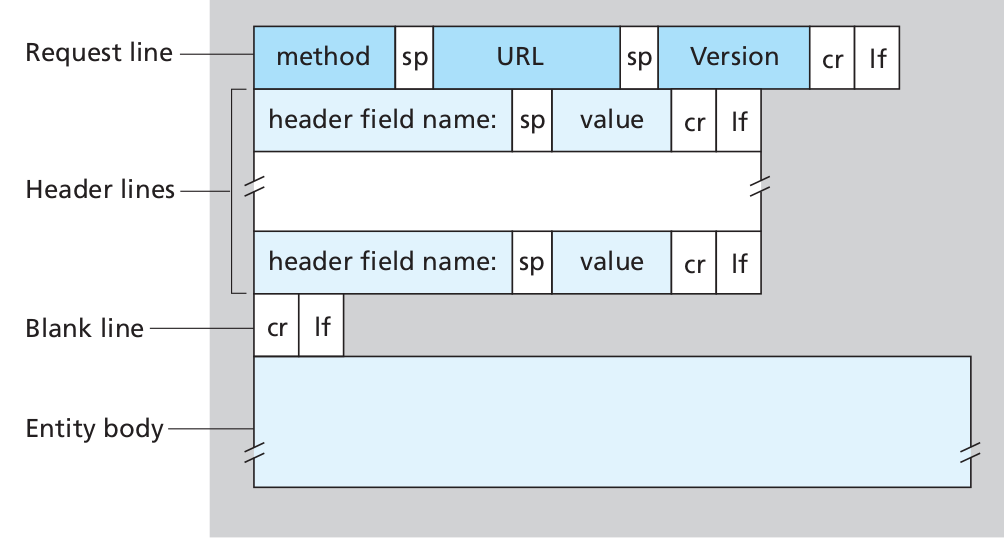
\includegraphics[width=0.5\textwidth]{Images/http_request}}
			\subfloat[HTTP Response Message]{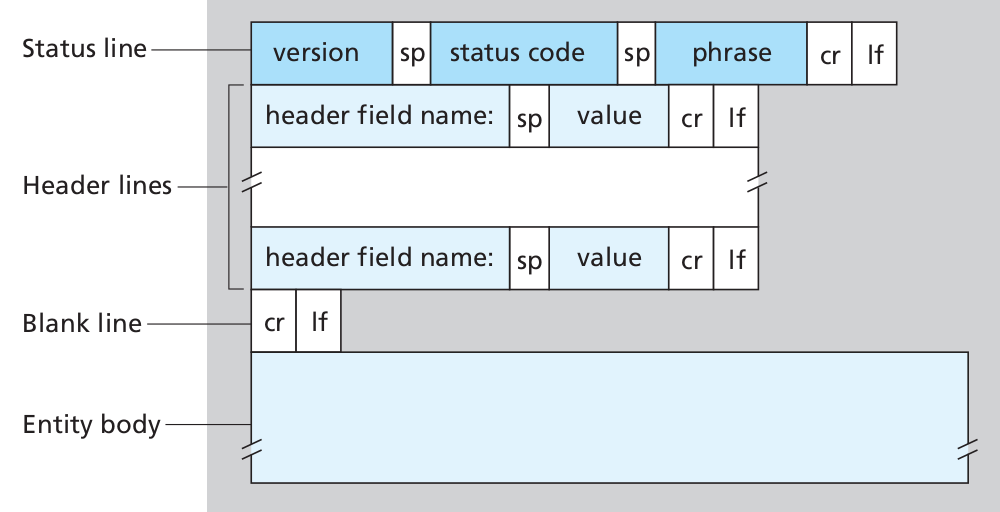
\includegraphics[width=0.5\textwidth]{Images/http_response}}
			\caption{HTTP Message Format}
		\end{figure}
		\vspace{-0.3cm}\item \textbf{TLSv1.2 :} TLSv1.2 is the successor of \textbf{SSL} and it provides communications security over a computer network. Symmetric cryptography is used to encrypt the data transmitted. The packet contains the type of message (handshake, alert, or data) in the '\textbf{Content Type}' field. It also contains the \textbf{version}, \textbf{length} of data and \textbf{MAC (Message Authentication Code)}.
		\begin{figure}[h]
			\centering
			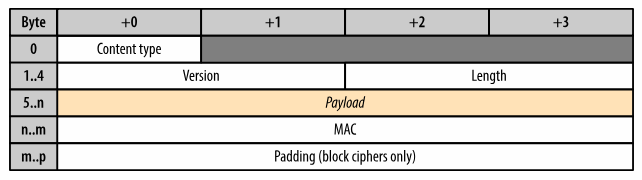
\includegraphics[width=0.7\textwidth]{Images/tls_message}
			\caption{TLSv1.2 Message Format}
		\end{figure}
	\end{itemize}
	\vspace{-0.3cm}\item \textbf{\color{Magenta} \large Transport Layer }\\
	\begin{adjustbox}{valign=T,raise=\strutheight,minipage={\linewidth}}
		\begin{wrapfigure}{r}{0pt}
			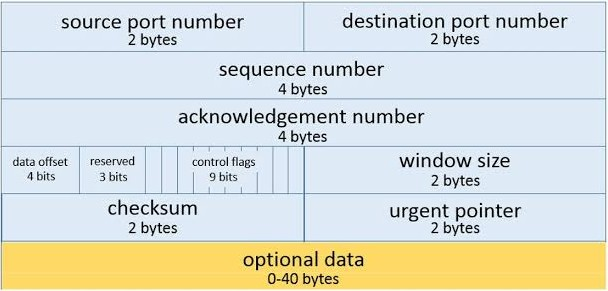
\includegraphics[width=10cm]{Images/tcp_segment}
			\caption{TCP Segment Format}
		\end{wrapfigure}
		\strut{}
		\textbf{Transmission Control Protocol} is a standard that defines how to establish and maintain a network conversation via which application programs can exchange data. \textbf{Source Port} and \textbf{Destionation Port} identify the hosts of the connection, source being the end point from where the segment is sent. \textbf{Sequence Number} specifies the number assigned to the first byte of data in the current message. If the ACK control bit is set, then \textbf{Acknowledgment number} refers to the next sequence number that the sender is expecting to receive. \textbf{Data offset} specifies the size of the variable sized TCP header. \textbf{Flags} are 1 bit values that specify the state of the connection and are used for control. \textbf{Window size} is the size of the buffer of the receiver. \textbf{Checksum} is used for error correction. Data field contains the payload of the segment.
	\end{adjustbox} 
	\item \textbf{\color{Magenta} \large Network Layer }\\
	\begin{adjustbox}{valign=T,raise=\strutheight,minipage={\linewidth}}
		\begin{wrapfigure}{l}{0pt}
			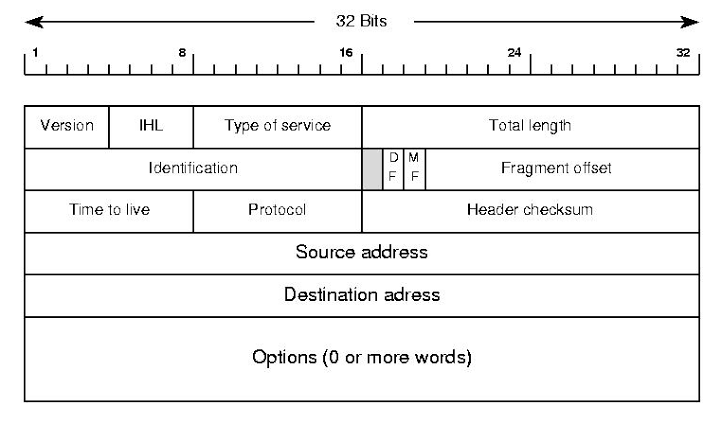
\includegraphics[width=10cm]{Images/ip_datagram}
			\caption{IP Datagram Header Format}
		\end{wrapfigure}
		\strut{}
		\textbf{IPv4 (Internet Protocol Version 4)} is one of the core protocols of standards-based internetworking methods in the Internet. It is used in packet-switched networks. Each IP datagram consists of a \textbf{header} and a \textbf{data} part. The header has a 20 byte fixed part followed by a variable-sized optional part. \textbf{Version} refers to the version of the datagram. In this case it would be 4. \textbf{IHL (Internet Header Length)} is the size of the header. \textbf{Types of Service} contains a 3-bit precedence field (that is ignored today), 4 service bits, and 1 unused bit. Service bits specify what characteristics the physical layer shhould use. \textbf{Total Length} is the total length of the datagram in bytes. \textbf{Identification} uniquely identifies the datagram. All fragments of a datagram contain the same identification value. \textbf{TTL (Time to Live)} is the maximum routers through which the segment can be switched. \textbf{Protocol} indicates the next higher level protocol that is contained within the data portion of the packet. \textbf{Header checksum} is used for error detection. \textbf{Source} and \textbf{destination addresses} are the addresses of the source and destination of the packet respectively.
	\end{adjustbox} 
	\item \textbf{\color{Magenta} \large Link Layer}\\
	\begin{adjustbox}{valign=T,raise=\strutheight,minipage={\linewidth}}
		\begin{wrapfigure}{r}{0pt}
			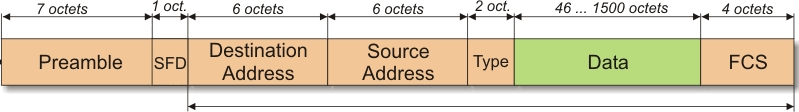
\includegraphics[width=12cm]{Images/ethernet_frame}
			\caption{Ethernet Frame Format}
		\end{wrapfigure}
		\strut{}
		\textbf{Ethernet II} is used in the link layer. \textbf{Preamble} is a 7 byte pattern of alternating 0's and 1's which indicates starting of the frame and allow sender and receiver to establish bit synchronization. \textbf{SFD} is the start frame delimiter and marks the start of frame. \textbf{Destination} and \textbf{source addresses} are the MAC addresses of the sending and receiving machines of the frame respectively. \textbf{Type} field is used to specify the protocol that is being used. \textbf{FCS (Frame Check Sequence)} is the error detecting code that is added. 
	\end{adjustbox} 
\end{enumerate}

\section*{Question 2: Observed Values in Different Protocols}
\begin{enumerate}[{\color{Magenta}A)}]
	\item \textbf{\color{Magenta} \large Application Layer}\\
	\begin{adjustbox}{valign=T,raise=\strutheight,minipage={\linewidth}}
		\begin{wrapfigure}{l}{0pt}
			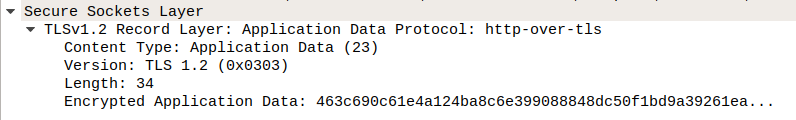
\includegraphics[width=10cm]{Images/AppEx}
			\caption{TLSv1.2 Record Example}
		\end{wrapfigure}
		\strut{}
		It is visible from the example that the appication data protocol is \textbf{Http-over-tls} (aka HTTPS). The \textbf{content type} in this message is Application Data. \textbf{Version }of TLS is 1.2. \textbf{Length} of the data is 34 bytes. \textbf{Encrypted Application Data} can also be seen. 
		\\HTTPS encrypts all message contents, including the HTTP headers and the request/response data, therefore no HTTP header or request/response can be seen explicitly.
	\end{adjustbox}
	\item \textbf{\color{Magenta} \large Transport Layer }\\
	\begin{adjustbox}{valign=T,raise=\strutheight,minipage={\linewidth}}
		\begin{wrapfigure}{r}{0pt}
			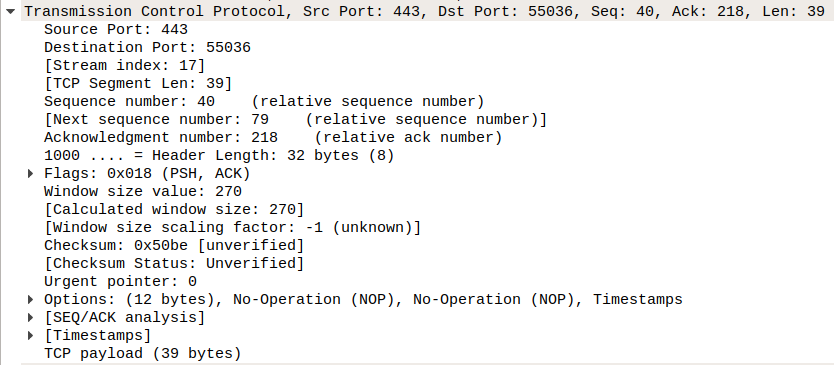
\includegraphics[width=10cm]{Images/TcpEx}
			\caption{TCP Segment Example}
		\end{wrapfigure}
		\strut{}
		It can be seen that the \textbf{source port} is 443 (This is to be expected because the default port for HTTPS connection is 443). The \textbf{destination port} is 55036. The \textbf{TCP Segment Length} is 39 bytes (payload). The \textbf{sequence number} is 40. \textbf{Acknowledgement number} is 218 which means that the sender of this segment is expecting a segment with sequence number 218 from the reciever. \textbf{Flags} field tells us that PSH and ACK flag is enabled. PSH flag is an option provided by TCP that allows the sending application to start sending the data even when the buffer is not full. \textbf{Window size} value is 270 (Number of packets sent before acknowledgment).	The \textbf{checksum} value can also be seen that is used for error detection.
	\end{adjustbox} 
	\pagebreak
	\item \textbf{\color{Magenta} \large Network Layer }\\
	\begin{adjustbox}{valign=T,raise=\strutheight,minipage={\linewidth}}
		\begin{wrapfigure}{l}{0pt}
			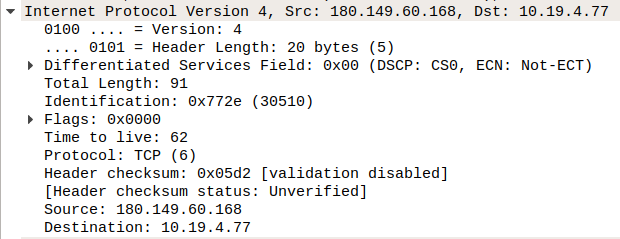
\includegraphics[width=10cm]{Images/IpEx}
			\caption{IP Datagram Example}
		\end{wrapfigure}
		\strut{}
		\textbf{Version} as stated earlier is 4 because IPv4 is being used. When IPv6 will be used, then the version will become 6. \textbf{Header Length} has the value 5 which implies that the header size is 20 bytes. \textbf{Total length} of the packet is 91 bytes and the \textbf{Identification number} is 0x772e. \textbf{Flag} value of 0000 implies that the datagram is not fragmented. \textbf{TTL} is 62 meaning that it can hop 62 times before dying. \textbf{Checksum} Value (0x05d2) can also be seen which is used for error detection. \textbf{Source address} (IP address of server) is 180.149.60.168. \textbf{Destination address} (IP address of my laptop) is 10.19.4.77
	\end{adjustbox} 
	\item \textbf{\color{Magenta} \large Link Layer }\\
	\begin{adjustbox}{valign=T,raise=\strutheight,minipage={\linewidth}}
		\begin{wrapfigure}{r}{0pt}
			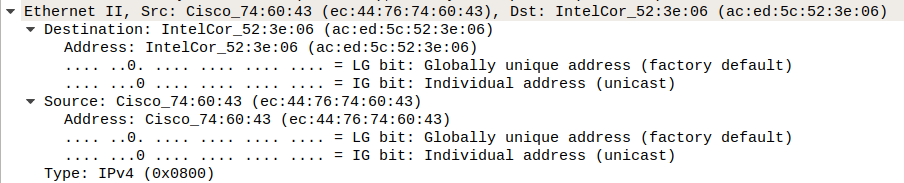
\includegraphics[width=12cm]{Images/linkEx}
			\caption{Ethernet Frame Example}
		\end{wrapfigure}
		\strut{}
		The information about the \textbf{Destination} and \textbf{Source MAC addresses} can be seen. They are unique addresses assigned to the \textbf{Network Interface controllers} of the machines. The source of this frame is a Cisco device and the destination is my laptop. The \textbf{Type} of connection can also be seen.
	\end{adjustbox} 
\end{enumerate}

\section*{Question 3: Observed Values in Different Protocols}
\end{document}
